% !TEX TS-program = xelatex
% !TEX encoding = UTF-8

% This is a simple template for a XeLaTeX document using the "article" class,
% with the fontspec package to easily select fonts.

\documentclass[11pt]{article} % use larger type; default would be 10pt

\usepackage{fontspec} % Font selection for XeLaTeX; see fontspec.pdf for documentation
\defaultfontfeatures{Mapping=tex-text} % to support TeX conventions like ``---''
\usepackage{xunicode} % Unicode support for LaTeX character names (accents, European chars, etc)
\usepackage{xltxtra} % Extra customizations for XeLaTeX

\setmainfont{CharisSIL} % set the main body font (\textrm), assumes Charis SIL is installed
\setsansfont{DejaVuSans}
\setmonofont{DejaVuSansMono}

% other LaTeX packages.....
\usepackage{geometry} % See geometry.pdf to learn the layout options. There are lots.
\geometry{letterpaper} % or letterpaper (US) or a5paper or....
%\usepackage[parfill]{parskip} % Activate to begin paragraphs with an empty line rather than an indent

\usepackage{graphicx} % support the \includegraphics command and options

\title{Brief Article}
\author{The Author}
\date{\today} % Activate to display a given date or no date (if empty),
         % otherwise the current date is printed 

\begin{document}
\maketitle

\section{Abstract}

A brief summary of the main points.

\section{Introduction}

Why did we do this?

\section{Materials and Methods}

How did we do this?

\section{Results and Discussion}

% 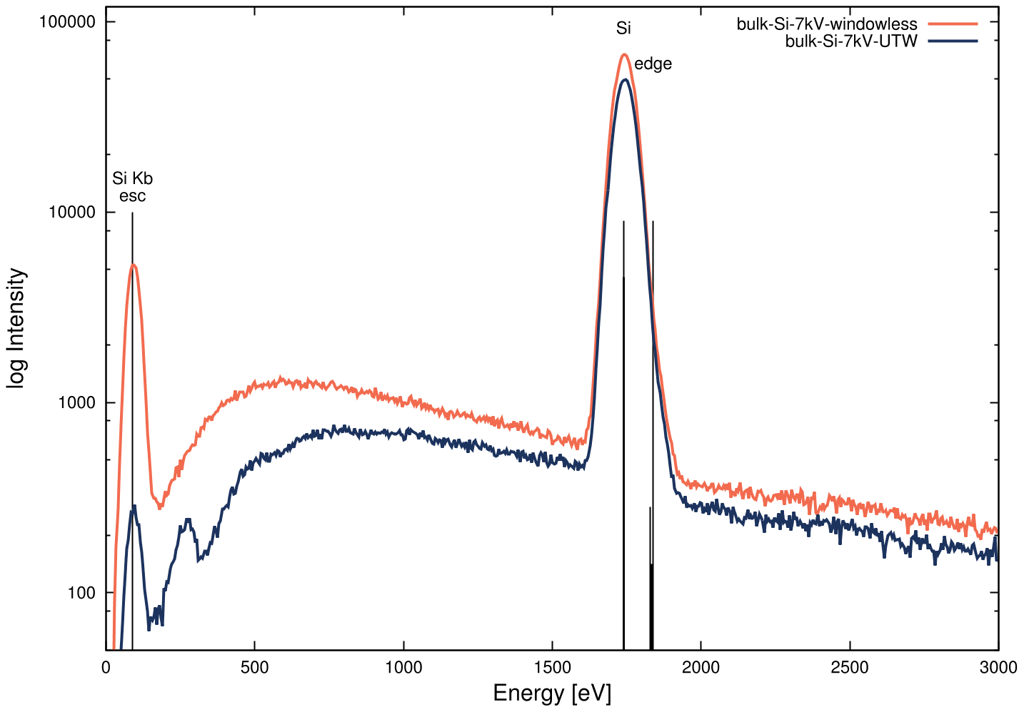
\includegraphics{figures/Si-at-7kV-window.png}
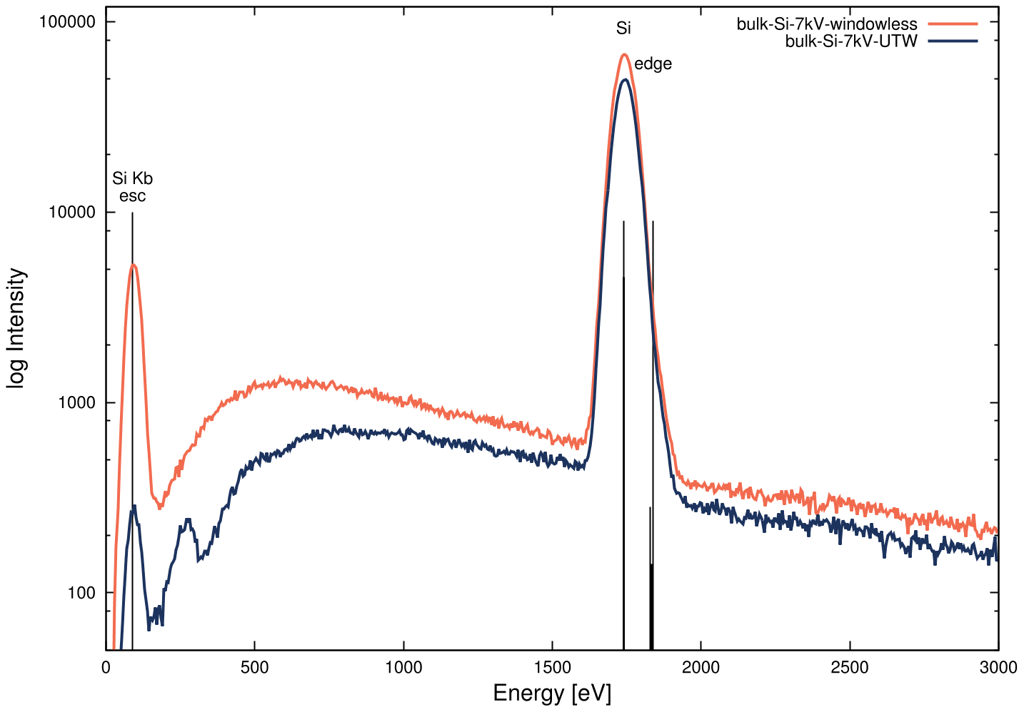
\includegraphics[width=6.5in,scale=0.125]{figures/Si-at-7kV-window.png}


Why was this worth documenting?

\section{Conclusions}

What did we conclude?

\section{Bibliography}

What references did we cite?





%\subsection{}



\end{document}